\chapter[Diseño del Hardware y Software del Sistema]{Diseño del Hardware y Software del Sistema.}

Este capitulo presenta el diseño del hardware y del software del sistema desarrollado. En la parte de hardware se habla de esto y esto. En la parte de software, se habla de esto y esto.

En la Figura~\ref{fig_bloque_c4} se presenta el diagrama en bloques simplificado del sistema, en dónde el principal componente es el microprocesador, que será alimentado por la batería del vehículo y se comunicará con el mismo mediante el transceiver CAN.  
Los datos obtenidos por el microprocesador serán procesados y enviados a un receptor por medio de un módulo inalámbrico, el receptor desplegará la información en un gráfico entendible para los usuarios del sistema. 
%%%%%%%%%%%%%%%%%%%%%%%%%%%%%%%%%%%%%%%%%%%%%%%%%%%%%%%%%%
\begin{figure}[H]
	\centering
		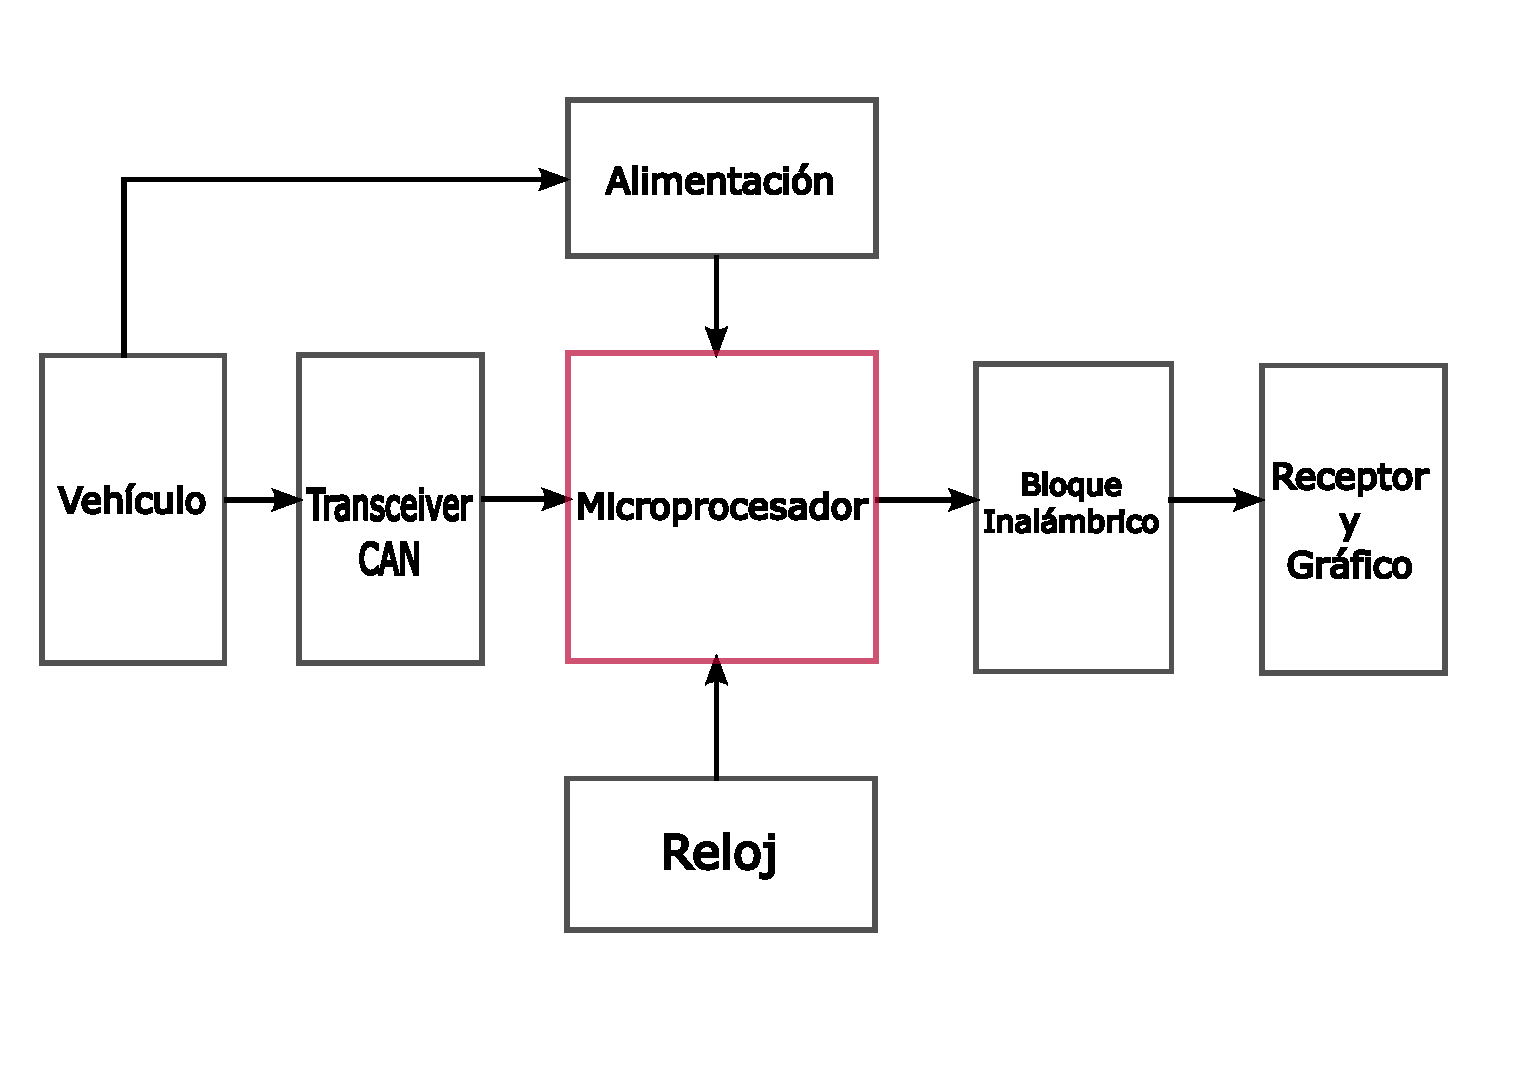
\includegraphics[width=0.9\textwidth]{./Cap4imagen/bloqueHardware.pdf}
	\caption[Diagrama en Bloque del sistema.]{Diagrama en Bloque del sistema.\textbf{ Fuente:}  Elaboración Propia.}
	\label{fig_bloque_c4} % Etiqueta para la referencia.
\end{figure}

% CITAR IMAGEN
%%%%%%%%%%%%%%%%%%%%%%%%%%%%%%%%%%%%%%%%%%%%%%%%%%%%%%%%%%


Para dicho diseño, se utilizará un microcontrolador de la familia PIC (\textit{Peripheral Interface Controller}, por sus siglas en inglés), ya que los PIC son una familia de microcontroladores con amplia documentación técnica y tiene una comunidad de personas activas utilizando estos microcontroladores. 
Son fabricados por \textit{Microchip Tecnhology Inc.} y existe una gran cantidad de modelos con características y prestaciones, esto nos permite escoger el modelo que se ajusta a la necesidad. 
Para el Proyecto se utilizó el PIC18F4580 que incluye internamente un módulo CAN y un módulo serial. 

\section{Diseño del Hardware con el PIC18F4580}
\subsection{Microcontrolador PIC18F4580}

Las características del módulo CAN incorporado en el PIC son las siguientes:
\begin{itemize}
	\item Aplicación del protocolo CAN 1.2,
	CAN 2.0A y CAN 2.0B.
	\item Tramas de datos estándar y extendidas.
	\item 0-8 bytes de longitud de datos.
	\item Tasa de bits programable hasta 1 Mbit / seg.
	\item Totalmente compatible con módulos CAN PIC18XXX8.
	\item Tres modos de funcionamiento:
	\begin{itemize}
		\item Modo 0: El modo tradicional.
		\item Modo 1: Mejora del modo tradicional con
		apoyo DeviceNet.
		\item Modo 2: Modo FIFO con el apoyo de DeviceNet.
		\end {itemize}
		\item Soporte para tramas remotas con el manejo automatizado.
		\item  Seis memorias intermedias programables como RX y TX, 
		almacenamientos intermedios de mensajes.
		\item 16 filtros de aceptancia.
		\item Dos máscaras de filtro de aceptancia completos que pueden ser asignado a cualquier filtro.
		\item Tres buffers de transmisión dedicados.
		\item Temporizador interno~\cite{DaP}.
		\item Modo de bajo consumo.
	\end{itemize}

Para que el PIC pueda realizar sus funciones es necesario programarlo y hemos de escribir un programa que contenga los procesos que el PIC debe ejecutar para manejar el módulo CAN y operar el protocolo. 
Este programa se puede escribir en varios lenguajes de programación, pero los  más utilizados son el ``Assembler'' (ensamblador) y el C. 
En el proyecto se utiliza el lenguaje C por su potencia y robustez para sistemas embebidos, para un último paso y traducir el programa a lenguaje máquina se utiliza el compilador  de CCS (\textit{Custom Computer Services, Inc.}, por sus siglas en inglés).

Otras características que se aprovecha del PIC18F4580 son: 
\begin{itemize}
\item {\textbf{Reloj:}} Ofrece varias opciones de configuración de la frecuencia de oscilación, permitiendo al usuario escoger según se adapte a sus necesidades.
Para la elección de la frecuencia de oscilación se ha escogido un clock de 16Mhz.
\item {\textbf{Input/Output:}} En este PIC hay 5 puertos diferentes (A, B, C, D y E). El diseño del hardware utiliza estos puertos para posibles expansiones del circuito o del sistema. 
\item {\textbf{Memoria de programa:}} Tiene 32 kbytes de memoria Flash, suficiente para el diseño del programa.
\item {\textbf{Periféricos:}} En el PIC18F4580 aprovechamos el módulo serial EUSART para comunicar los datos procesador a una central~\cite{DaP}.

\end{itemize}


\subsection{Transceiver BUS CAN MCP2551}
El módulo CAN del  PIC18F4580 precisa de un componente externo llamado transceiver CAN. 
Esto es así para proteger el microcontrolador de cortocircuitos o sobretensiones. 
Los transceiver están diseñados para uso en aplicaciones de comunicación BUS CAN en la capa física según la norma ISO 11898. 
El transceiver proporciona una transmisión y recepción de bus diferencial para el controlador CAN y ofrece velocidades de hasta 1Mbps.
El MCP2551 está diseñado para funcionar en ambientes agresivos y cuenta con protección contra sobretensiones, sobrecalentamiento y una amplia gama de modos de servicios. 
El pin 8 ofrece tres modos de funcionamiento: alta velocidad, control de pendiente, y modos de bajo consumo.
El modo de alta velocidad de funcionamiento se selecciona mediante la conexión del PIN 8 a tierra, permitiendo a los transistores de salida del transmisor encender y apagar lo más rápido posible. 
En este proyecto utiliza este modo de funcionamiento.

Las pendientes de subida y bajada de los bits se pueden ajustar mediante la conexión de una resistencia a tierra en el PIN 8, ya que la pendiente del bit es proporcional a la corriente de salida del PIN. 
Este control de la pendiente se implementa aplicando valores a la resistencia externa en el PIN 8. 
Por ejemplo con una resistencia de 10 kohm se logra una pendiente de bit de 15V/us,  y con una resistencia de 100 kohm se logra una pendiente de bit de 2V/us. 
Si se aplica un nivel lógico alto al PIN 8 el transceiver entra en modo standby, para ahorrar energía y vuelve a su estado de trabajo al aplicar un nivel lógico bajo al PIN 8. El pin $V_{ref}$ 5 está disponible como una referencia de tensión~\cite{sn}.

\subsection{Módulos inalámbricos Xbee}
 los módulos XBee son soluciones integradas que brindan un medio inalámbrico para la interconexión y comunicación entre dispositivos. Estos módulos utilizan el protocolo de red llamado IEEE 802.15.4 para crear redes POINT-TO-MULTIPOINT (punto a multipunto); o para redes PEER-TO-PEER (punto a punto). Fueron diseñados para aplicaciones que requieren de un alto tráfico de datos, baja latencia y una sincronización de comunicación predecible~\cite{xbee_c4}, en la Figura ~\ref{fig_xbee_4} observamos su apariencia. 
 
 %%%%%%%%%%%%%%%%%%%%%%%%%%%%%%%%%%%%%%%%%%%%%%%%%%%%%%%%%%
\begin{figure}[H]
	\centering
		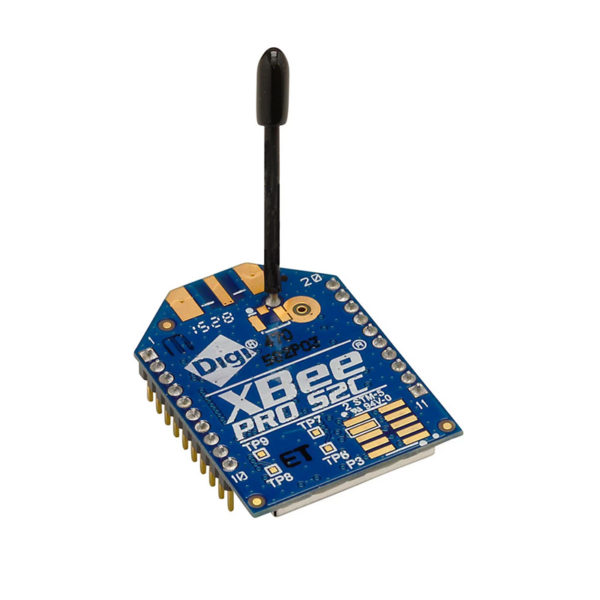
\includegraphics[width=0.6\textwidth]{./Cap4imagen/xbee_modulo.jpg}
	\caption[Fuente de Alimentación.]{Fuente de Alimentación.\textbf{ Fuente:}  \cite{cite_xbee_4}.}
	\label{fig_xbee_4} % Etiqueta para la referencia.
\end{figure}

% CITAR IMAGEN
%%%%%%%%%%%%%%%%%%%%%%%%%%%%%%%%%%%%%%%%%%%%%%%%%%%%%%%%%%

\subsection{Diseño del Hardware}
El montaje implementado es una placa de hardware BUS CAN, basado en el microcontrolador de bajo coste PIC18F4580. La función principal del mismo, es poder leer datos del BUS
CAN y enviarlos a un servidor para mostrarlos en una interfaz gráfica. 
Para realizar la placa PCB (\textit{Printed Circuit Board}, por sus siglas en inglés) se utilizó el software Proteus~\cite{pro},  el cual es un programa de diseño de diagramas y PCBs con autoenrutador. 
Proteus tiene una facilidad de uso y configuración.

En la Figura~\ref{Esch1} se observa el diagrama del bloque de alimentación del hardware que cuenta con un regulador de tensión LM7805 y dos condensadores electrolíticos cuya función es eliminar el rizado de la señal en la entrada del regulador para que la tensión de salida no tenga variaciones de tensión debido a irregularidades de la fuente principal. 

%%%%%%%%%%%%%%%%%%%%%%%%%%%%%%%%%%%%%%%%%%%%%%%%%%%%%%%%%%
\begin{figure}[H]
	\centering
		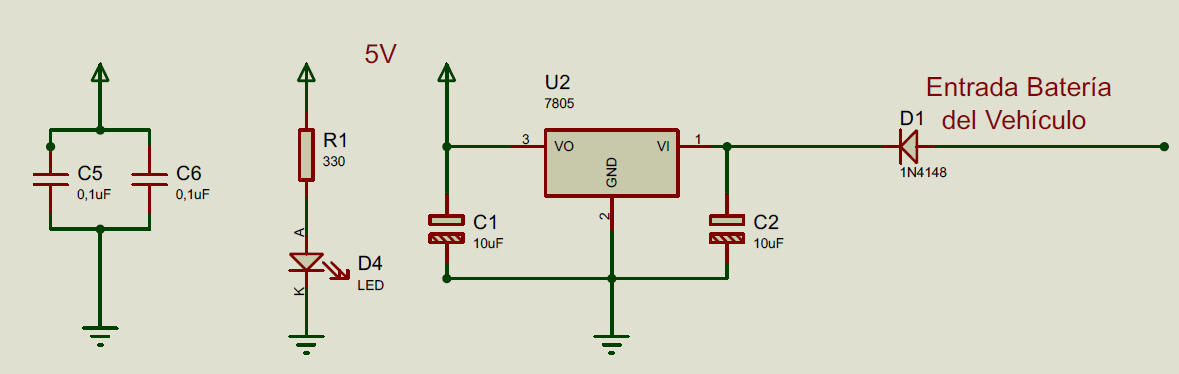
\includegraphics[width=0.6\textwidth]{./Cap4imagen/Fuente5v_4.png}
	\caption[Fuente de Alimentación.]{Fuente de Alimentación.\textbf{ Fuente:} 
	%\cite{sch1}.
	Elaboración Propia.}
	\label{Esch1} % Etiqueta para la referencia.
\end{figure}

% CITAR IMAGEN


%%%%%%%%%%%%%%%%%%%%%%%%%%%%%%%%%%%%%%%%%%%%%%%%%%%%%%%%%%

El Transceiver MCP2551 de Microchips es una interfaz entre el controlador del protocolo BUS CAN que se encuentra en el PIC, y el BUS CAN físico. 
Este chip está formado por un driver que nos convierte las señales que entran por el CANH  y CANL a señales CMOS para tener una lectura correcta de los datos en el PIC. 
La configuración de pines no requiere otros elementos aparte de los propios conectores para  entrada, salida y fuente de alimentación. 
En la Figura~\ref{Esch2} se observa la conexión donde el PIC será el nodo maestro encargado de escanear y procesar los datos provenientes del bus mediante la ayuda del transceiver CAN. 
La misma se conectará a un conector OBD II mediante un conector DB9. 
La alimentación proviene del conector DB9 que irá a extraer la energía de la batería del vehículo.


%%%%%%%%%%%%%%%%%%%%%%%%%%%%%%%%%%%%%%%%%%%%%%%%%%%%%%%%%%%
\begin{figure}[H]
	\centering
		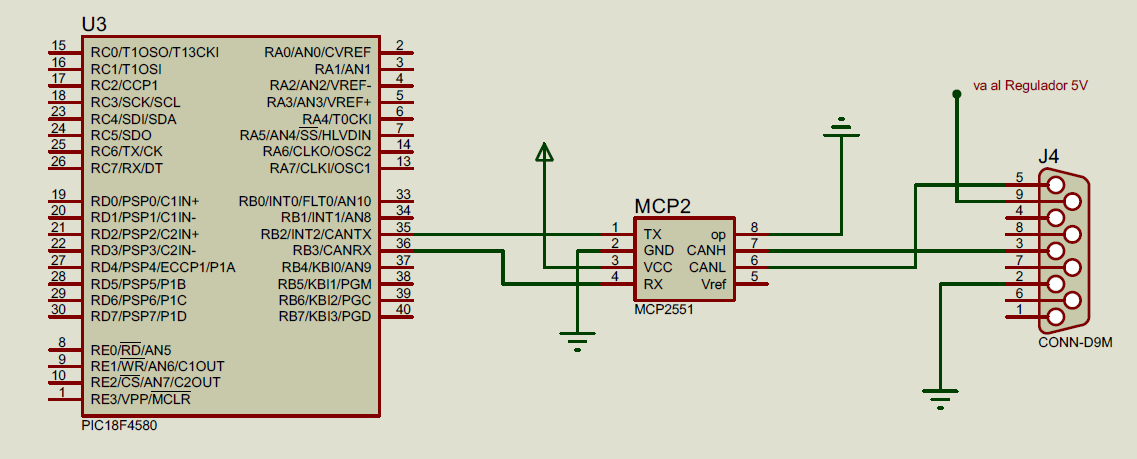
\includegraphics[width=0.9\textwidth]{./Cap4imagen/pic_y_mcp_4.png}
	\caption[Esquemático del Transceiver CAN.]{Esquemático del Transceiver CAN.\textbf{ Fuente:} 
		%\cite{Tu}.
		Elaboración propia}
	\label{Esch2} % Etiqueta para la referencia.
\end{figure}

% CITAR IMAGEN


%%%%%%%%%%%%%%%%%%%%%%%%%%%%%%%%%%%%%%%%%%%%%%%%%%%%%%%%%%%

En la Figura~\ref{Esch3} se observa la incorporación de un módulo inalámbrico Xbee para la comunicación con el servidor de datos. 


%%%%%%%%%%%%%%%%%%%%%%%%%%%%%%%%%%%%%%%%%%%%%%%%%%%%%%%%%%%%%
\begin{figure}[H]
	\centering
		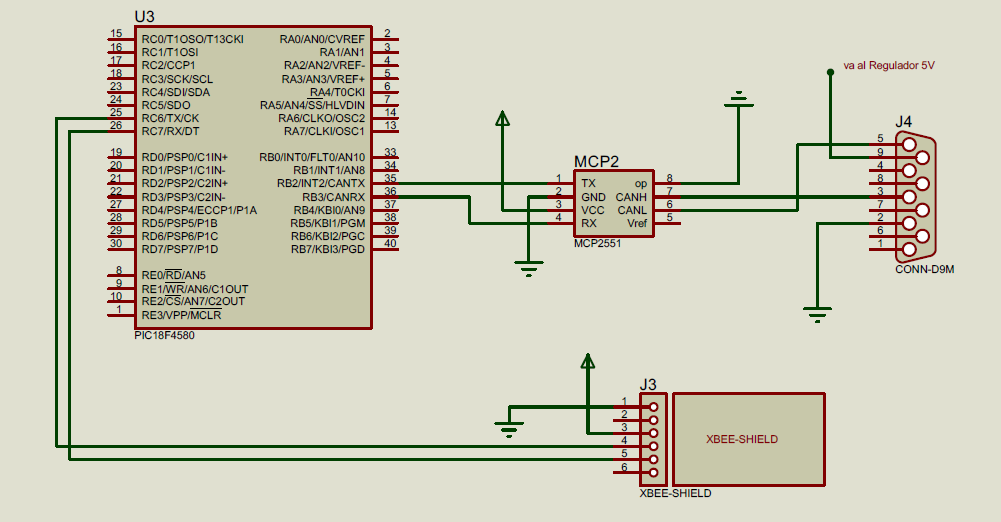
\includegraphics[width=0.9\textwidth]{./Cap4imagen/xbee_4.png}
	\caption[Esquemático PIC y Módulo inalámbrico Xbee.]{Esquemático PIC y Módulo inalámbrico Xbee.\textbf{Fuente:} Elaboración propia.}
	\label{Esch3} % Etiqueta para la referencia.
\end{figure}

% CITAR IMAGEN


%%%%%%%%%%%%%%%%%%%%%%%%%%%%%%%%%%%%%%%%%%%%%%%%%%%%%%%%%%%%%
 En la Figura~\ref{Esch5} que presenta el circuito completo se puede observar los bloques principales del diseño, el bloque de programación y $reset$, el bloque de alimentación y regulación que es alimentado por la batería de 12v del vehículo y luego es reducida a 5v, el bloque de reloj el cual nos da el clock necesario para configurar la velocidad del bus CAN, el bloque inalámbrico para la comunicación a distancia, el bloque transceiver CAN y el bloque de entrada del vehículo. 
 

%%%%%%%%%%%%%%%%%%%%%%%%%%%%%%%%%%%%%%%%%%%%%%%%%%%%%%%%%%%%%

%%%Las distancias indicadas son trim = izquierda abajo
%%%derecha arriba, y debe ir siempre seguido del comando clip.
\begin{figure}[H]
	\centering
		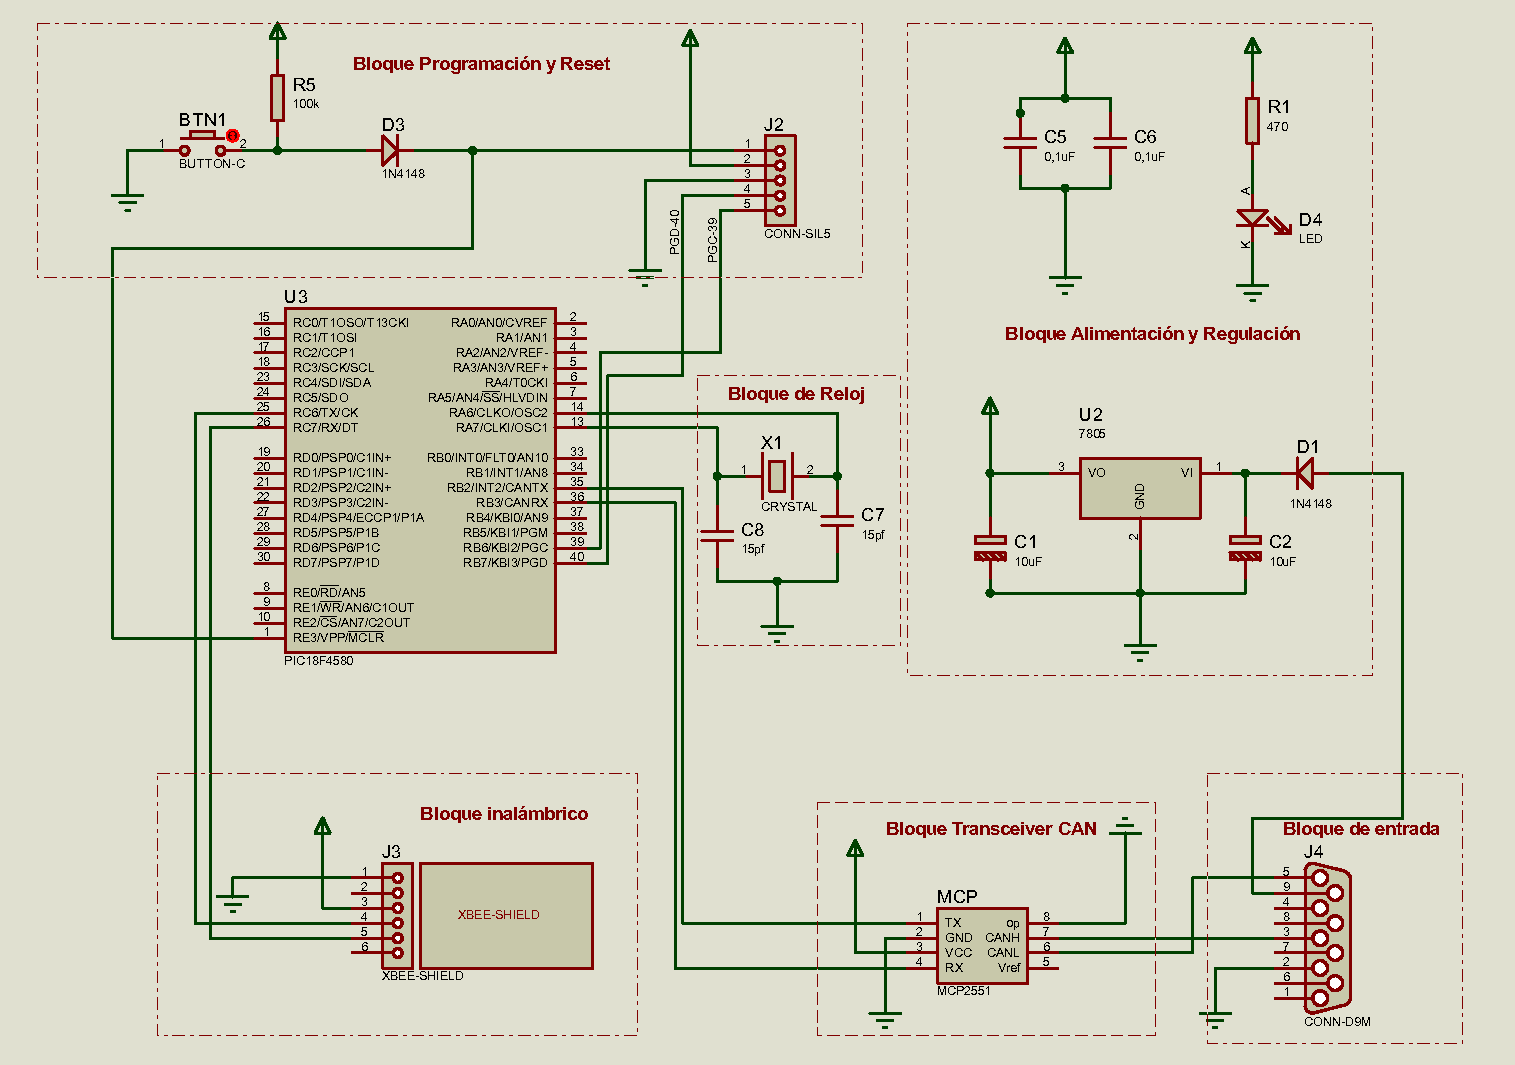
\includegraphics[ width=1\textwidth]{./Cap4imagen/ctocompleto_4.pdf}
	\caption[Diseño del Circuito completo BUS CAN.]{Diseño del Circuito completo BUS CAN.\textbf{ Fuente:} Elaboración propia.}
	\label{Esch5} % Etiqueta para la referencia.
\end{figure}

% CITAR IMAGEN
 En la figura Figura~\ref{Esch6} se puede ver la imagen en PCB y en la que se observa la distribución de los componentes electrónicos en la placa.
%%%%%%%%%%%%%%%%%%%%%%%%%%%%%%%%%%%%%%%%%%%%%%%%%%%%%%%%%%%%%
\begin{figure}[H]
	\centering
		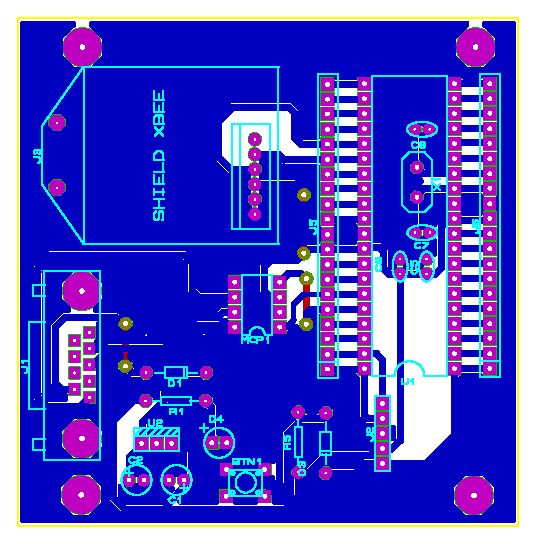
\includegraphics[ width=0.7\textwidth]{./Cap4imagen/pcb_can_4.pdf}
	\caption[ Apariencia del diseño PCB.]{Apariencia del diseño PCB.\textbf{ Fuente:} Elaboración Propia.}
	\label{Esch6} % Etiqueta para la referencia.
\end{figure}

% CITAR IMAGEN


%%%%%%%%%%%%%%%%%%%%%%%%%%%%%%%%%%%%%%%%%%%%%%%%%%%%%%%%%

En la Figura~\ref{Esch7} se muestra las vistas 3D del circuito impreso y ensamblado. 

%%%%%%%%%%%%%    TRANSEIVER         %%%%%%%%%%%%%%%%%%%
\begin{figure}[H]
	\centering
		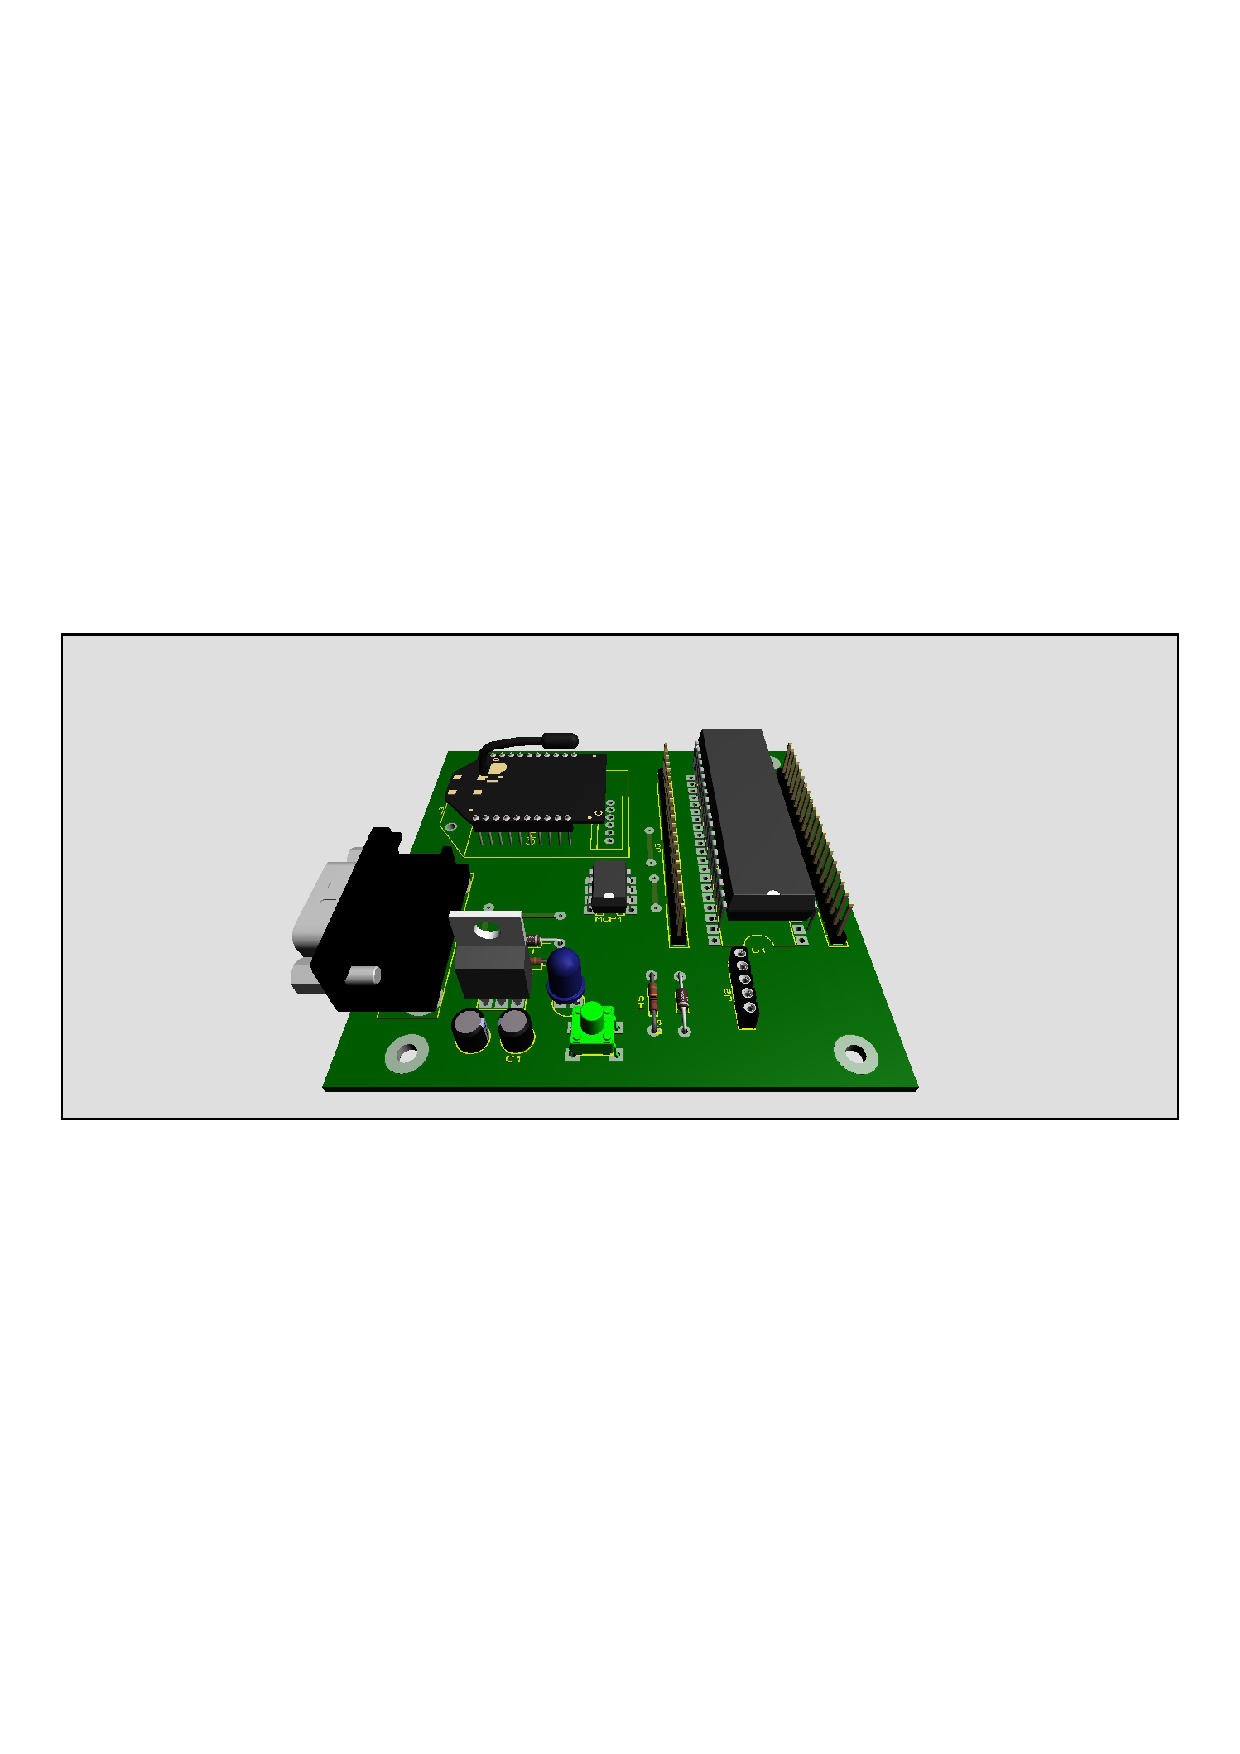
\includegraphics[trim = 10mm 60mm 5mm 50mm, clip, width=0.5\textwidth]{./Cap4imagen/3d_can_4.pdf}
	\caption[Vista 3D del Hardware.]{Vista 3D del Hardware.\textbf{ Fuente:} Elaboración propia.}
	\label{Esch7} % Etiqueta para la referencia.
\end{figure}

% CITAR IMAGEN
%%%%%%%%%%%%%%%%%%%%%%%%%%%%%%%%%%%%%%%%%%%%%%%%%%%%%%%%%%%%%

%%%%%%%%%%%%%%%%%%%%%%%%%%%%%%%%%%%%%%%%%%%%%%%%%%%%%%%%%
\subsection{Proceso de Construcción}
%%%%%%%%%%%%%%%%%%%%%%%%%%%%%%%%%%%%%%%%%%%%%%%%%%%%%%%%

Una vez obtenido el diseño del circuito se procedió a utilizar la máquina CNC (Control Numérico Computarizado)  de la marca Cirqoid para la fabricación del prototipo. 
Este equipo se encuentra en el laboratorio de Sistemas Distribuidos de la FIUNA. 
La CNC Cirqoid se encarga de realizar circuitos eléctricos automáticamente  pudiendo realizar los procesos de desgaste de cobre en una PCB, perforado, dispensación de la pasta de soldar y la colocación componentes electrónicos de tipo SMD (Dispositivos de Montaje Superficial, por sus siglas en inglés) , tomando en cuenta que para cada uno de estos procesos tiene su propio cabezal de trabajo~\cite{cirq}. 
En la Figura~\ref{Esch8} se observa la apariencia del sistema y la elaboración de la placa. 

\begin{figure}[H]
	\centering
		\includegraphics[width=0.7\textwidth]{./Cap4imagen/fresado_4.jpg}
	\caption[Proceso de fabricación del circuito PCB con la máquina CNC.]{Proceso de fabricación del circuito PCB con la máquina CNC.\textbf{ Fuente:} Elaboración propia.}
	\label{Esch8} % Etiqueta para la referencia.
\end{figure}

% CITAR IMAGEN


%%%%%%%%%%%%%%%%%%%%%%%%%%%%%%%%%%%%%%%%%%%%%%%%%%%%%%



%###############################################################################
Una vez culminado el proceso en la Figura~\ref{Esch9} se presenta la placa pcb terminada. 


\begin{figure}[H]
	\centering
	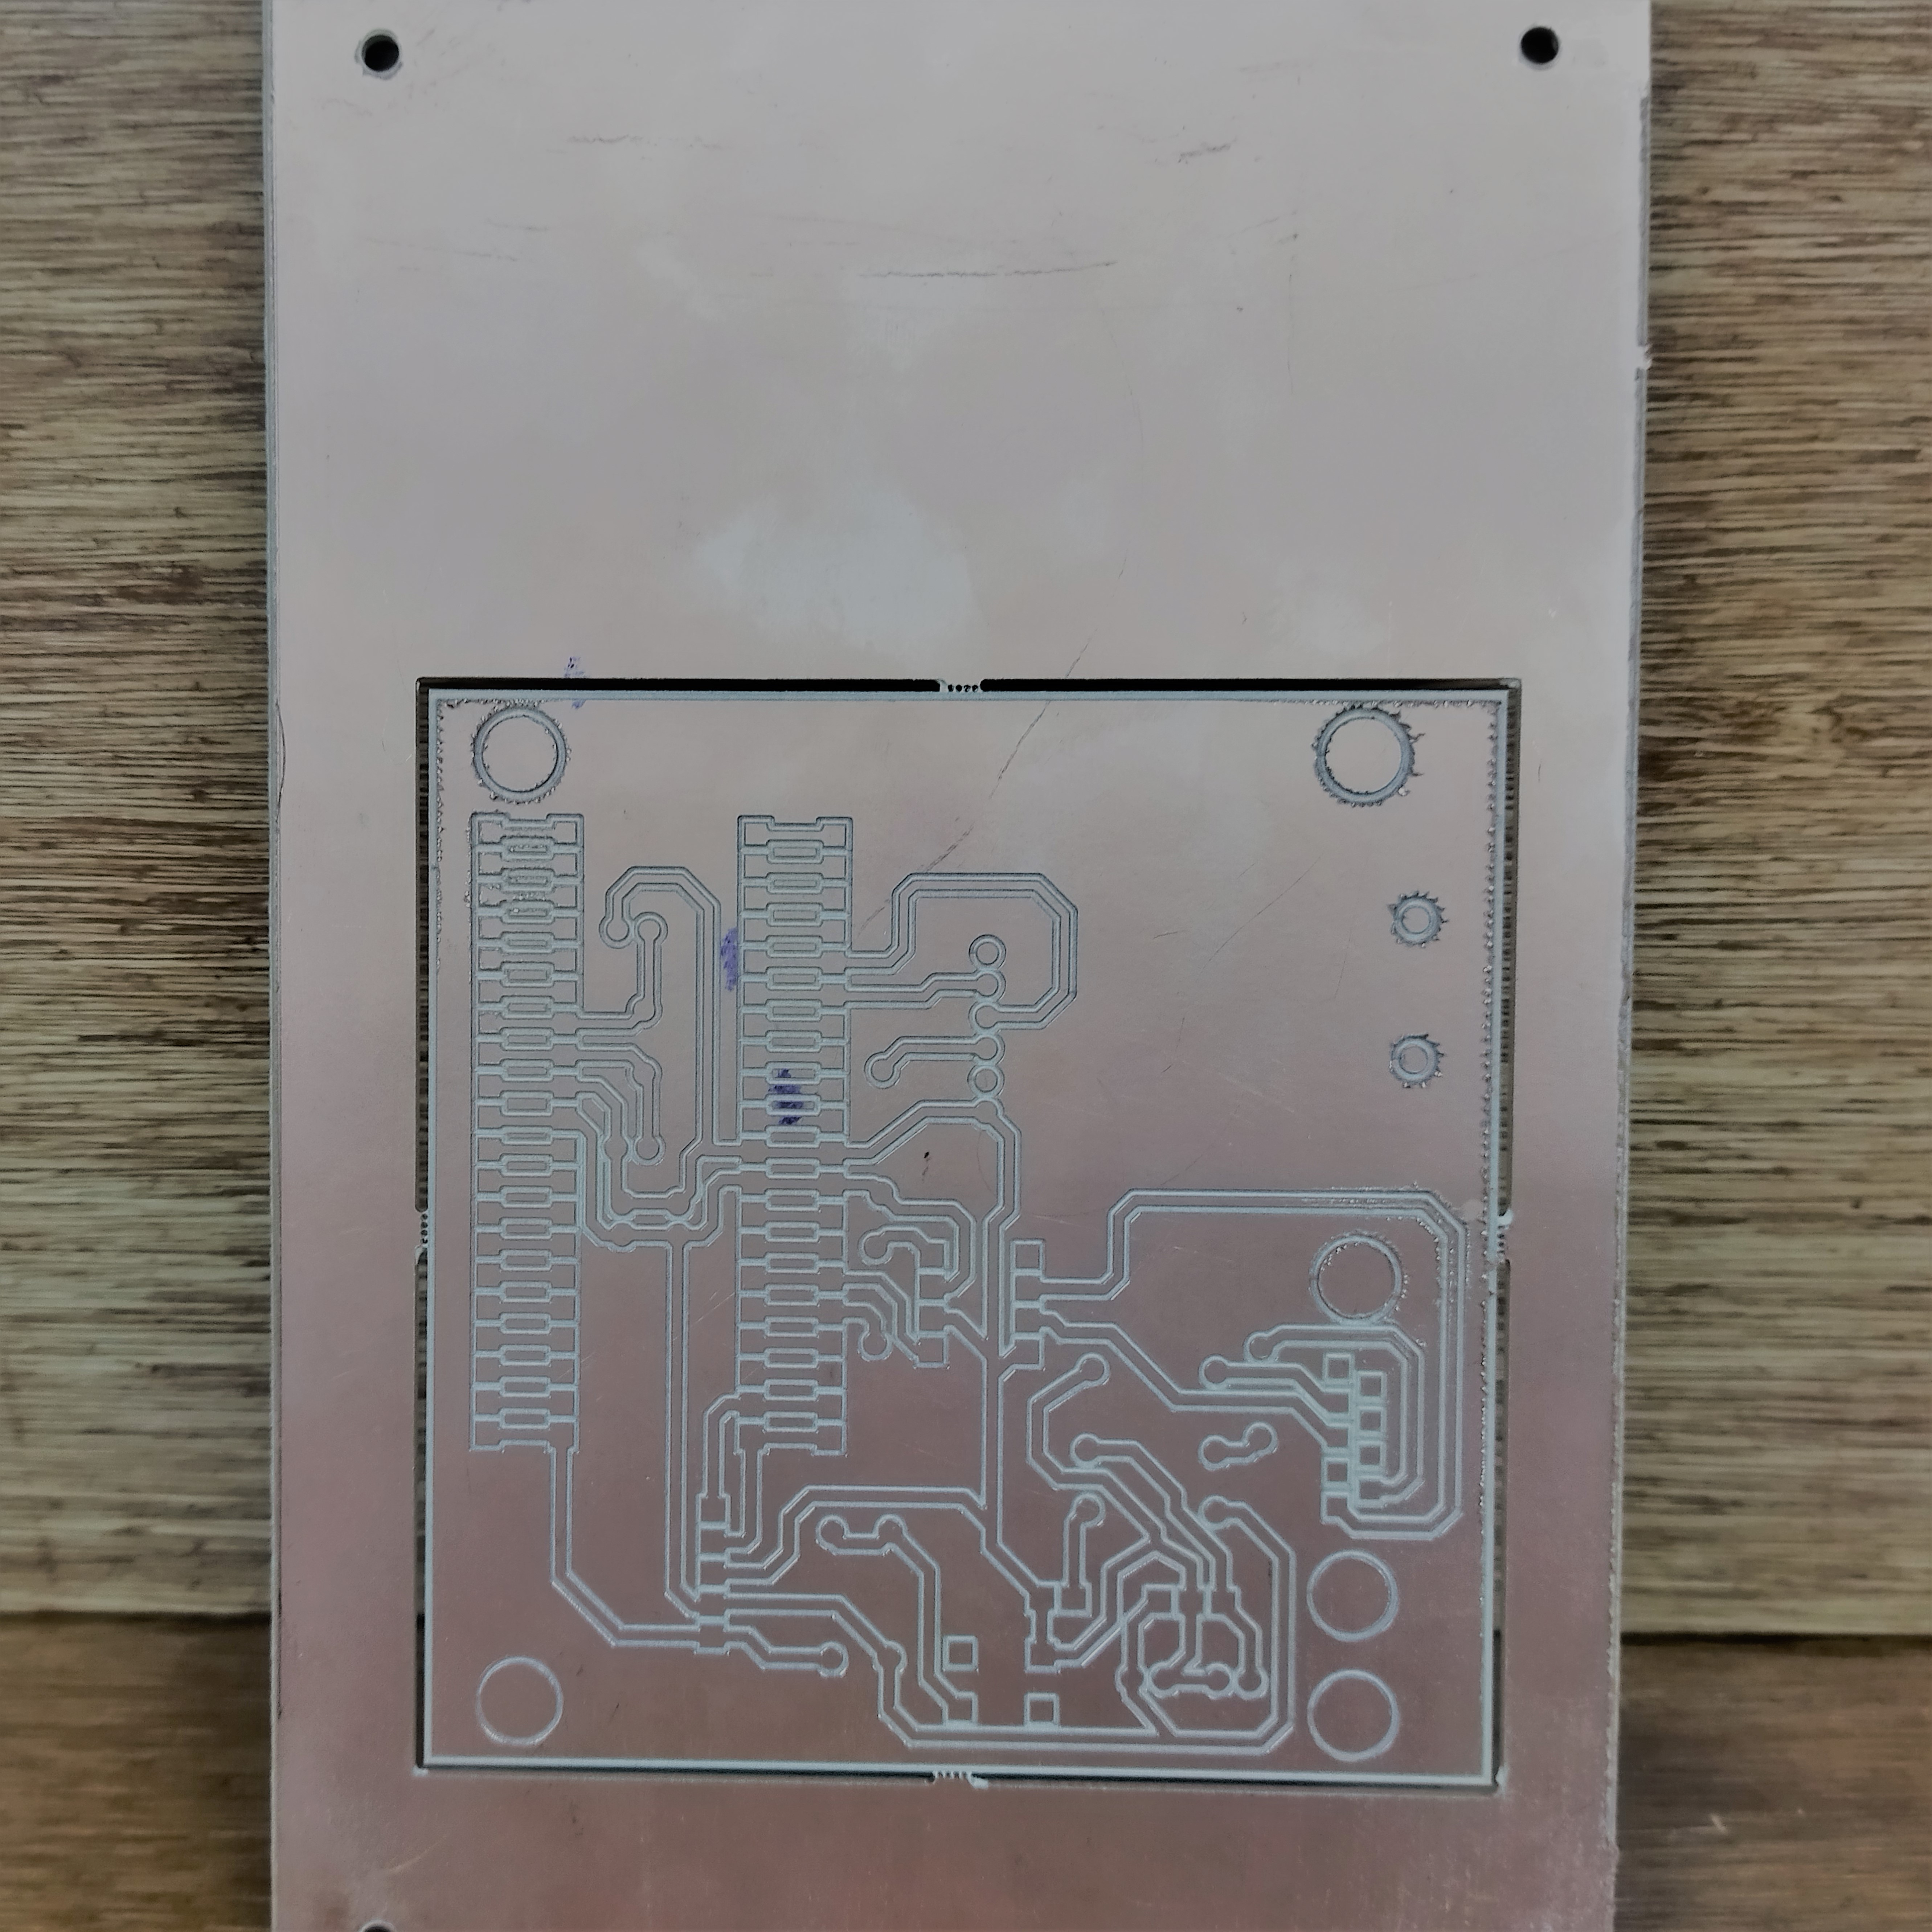
\includegraphics[width=0.5\textwidth]{./Cap4imagen/placa_pcb_4.jpg}
	\caption[Placa impresa.]{Placa impresa. \textbf{ Fuente:} Elaboración propia.}
	\label{Esch9} % Etiqueta para la referencia.
\end{figure}
%###############################################################################

Una vez obtenida el diseño de las pistas del circuito en la placa PCB, se procedió al ensamblado de la misma, resultando el hardware ilustrado en la siguiente Figura~\ref{Esch10}.


%###############################################################################
 
\begin{figure}[H]
	\centering
	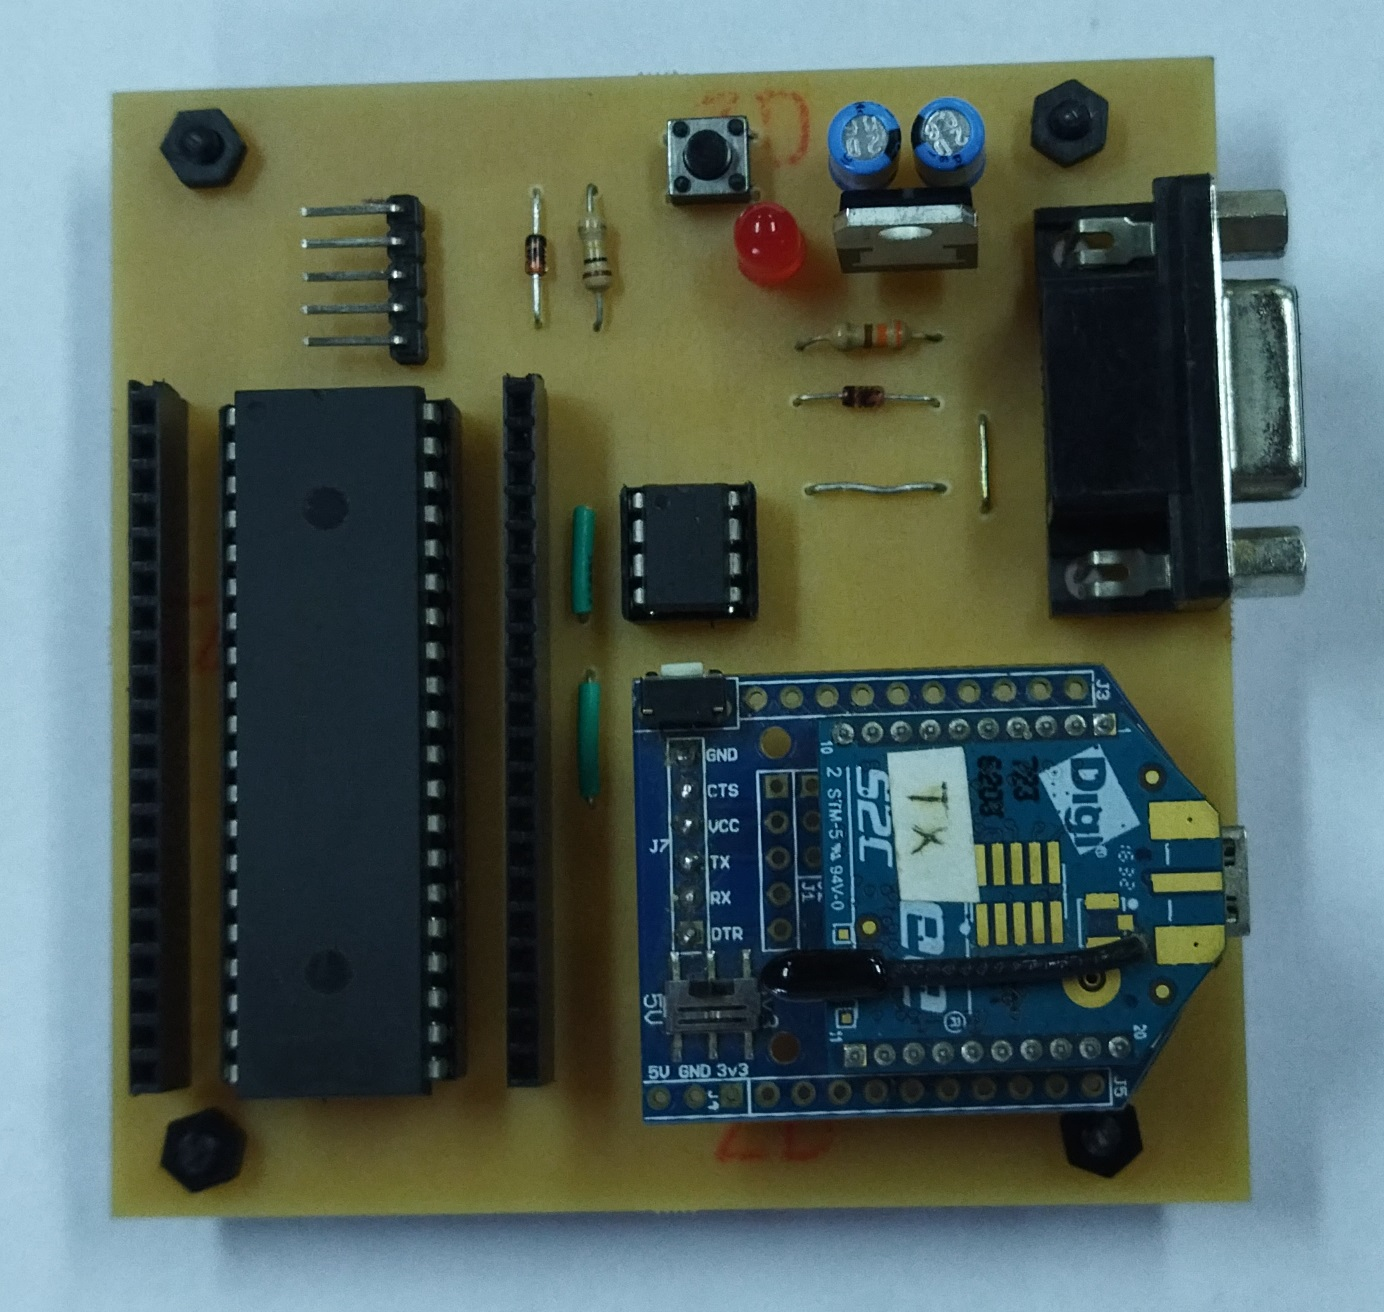
\includegraphics[width=0.5\textwidth]{./Cap4imagen/cto_ensamblado_4.jpg}
	\caption[Vista del Hardware ensamblado.]{Vista del Hardware ensamblado.\textbf{ Fuente:} Elaboración propia.}
	\label{Esch10} % Etiqueta para la referencia.
\end{figure}
%###############################################################################

%%%%%%%%%%%%%%%%%%%%%%%%%%%%%%%%%%%%%%%%%%%%5
%%%%%%%%% SIGUIENTE EXcAPITULO 5

%\chapter[Capítulo 5. Diseño del Software]{Diseño del Software}

\section {Diseño del Software del Sistema OBD II y J1939}
Para el diseño del sistema se recurrieron a las siguientes herramientas 
\begin{itemize}
    \item \textbf{IDE PIC CCS: } Para la programación del PIC18F4580 se utilizó como entorno de desarrollo el PIC CCS, que es un entorno de programación en lenguaje C que ya incluye además el compilador del lenguaje \cite{ccs}. 
    
    \item \textbf{Visual Studio Code:} Visual Studio Code es un editor de código fuente y entorno de desarrollo ligero que se ejecuta en un escritorio Windows, macOS y Linux. 
    Viene con soporte incorporado para JavaScript y  Node.js \cite{vsc}, el desarrollo del sistema de visualización OBD II y J1939 se trabaja en Visual Studio Code, facilitando el trabajo tanto para el desarrollo del cliente como del servidor. 
	\item {\bfseries Node.js: }	Node.js es un entorno de ejecución para JavaScript construido con el motor de JavaScript V8 de Chrome, fue ideado como un entorno de ejecución de JavaScript orientado a eventos asíncronos y está diseñado para crear aplicaciones network escalables, para una aplicación dada con esta herramienta puede atenderse muchas conexiones simultáneamente.
	HTTP es un elemento destacado en Node.js, diseñado teniendo en cuenta la transmisión de operaciones con \textit{streaming} y baja latencia. 
	Esto hace que Node.js sea muy adecuado para la base de una librería o un framework web~\cite{nodejs}.
	%Fuente: https://nodejs.org/es/about/
	\item {\bfseries Express.js: } es una infraestructura web rápida, minimalista y flexible para las aplicaciones Node.js. ``Express es una infraestructura de aplicaciones web Node.js minimalista y flexible que proporciona un conjunto sólido de características para las aplicaciones web y móviles. 	
	Con miles de métodos de programa de utilidad HTTP y middleware a su disposición, la creación de una API sólida es rápida y sencilla. 
	Express proporciona una delgada capa de características de aplicación web básicas, que no ocultan las características de Node.js"~\cite{express}. %[https://expressjs.com/es/resources/glossary.html]
	\item {\bfseries Socket.IO: } ``es una biblioteca que permite la comunicación en tiempo real, bidireccional y basada en eventos entre el navegador y el servidor. 
	Consiste en  un servidor Node.js y una biblioteca cliente de Javascript para el navegador"~\cite{socket}. %[ https://socket.io/docs/v4]
	\item {\bfseries Bootstrap: } ``Es un marco de desarrollo que facilita la construcción de páginas web desde el punto de vista estético", \cite{boot}. %[https://getbootstrap.com/]
	\item {\bfseries AdminLTE: } ``Es un diseño de presentación  de código abierto que ofrece un  panel de administración y  un panel de control para la visualización de una página web. 
	Construido sobre Bootstrap, AdminLTE proporciona una gama de componentes receptivos, reutilizables y de uso común"~\cite{admin}. %https://adminlte.io/
	
	Para el diseño de presentación de los datos OBDII y J1939 se utiliza dicha librería por su aspecto amigable desde el punto de vista de un usuario particular. 
	Esta librería solo nos proporciona el diseño de la parte visual y no los algoritmos necesarios para observar la dinámica de las mediciones del vehículo motor, para ello tratamos los datos con el lenguaje javascript. 
	
	\item {\bfseries Canvas-gauge.js:} son componentes minimalistas de código abierto basados en HTML5 para aplicaciones web que simulan un entorno de medidores analógicos. 
	Los medidores  se pueden instalar simplemente usando el administrador de paquetes de nodejs. ``Dependiendo de sus necesidades, existe la posibilidad de instalar una biblioteca de medidores completa o solo la parte que realmente necesita para su proyecto"~\cite{gauge}. %[ https://canvas-gauges.com/]
	
\end{itemize}


\subsection{Diseño del Firmware para el sistema OBDII}

Para mostrar la secuencia de funcionamiento se presenta en la siguiente  Figura~\ref{sobd} un diagrama de secuencia. 
El sistema inicializa el módulo CAN BUS con {\bfseries can-init()} y se habilita las interrupciones del módulo serial y las banderas de interrupciones globales con la función {\bfseries serial-isr()}. 
La interrupción del módulo serial permitirá avisar al microcontrolador cuando los datos recibidos desde un cliente desean consultar datos del bus. 
Este valor es almacenado en la trama CAN para enviarla al sistema del automóvil.

Con la inicialización del módulo CAN bus se procede a configurar los filtros del protocolo, pues nos permitirá recibir solo los datos que nos interesan e ignorará los que no nos sirven, para el Protocolo OBDII permitiremos que solamente leamos las respuesta que nos da la computadora. 
De manera estándar la computadora del vehículo envía mensajes con el siguiente rango de identificadores: 0x7E0 a 0x7E8. 

Una vez tenemos esto podemos proceder a la consulta enviando una trama CAN al bus con la función {\bfseries can-putd(id, data)} y se espera a que el sistema vehicular nos responda. 
Al recibir la respuesta del sistema auto motor con la función {\bfseries cant-getd(id,data)} dichos datos pasan por un procesamiento para interpretar los bits recibidos en los campos de datos. 
Para ello se utiliza los documentos OBD-II SAE J1979 donde indica los procedimientos matemáticos para el calculo de las mediciones. 

Luego se envía dichos datos a nuestro servidor con la función {\bfseries print()}. 
El formato de envío de mensaje se llama JSON, es un tipo de formato para el intercambio de datos entre software basado en texto y se utiliza mucho para el desarrollo web. 
Esto permitirá que en el lado del servidor podamos manipular mejor los datos enviados por el PIC: 

\{
	''A'':  00, 
	''B'': 11, 
	''C'': 22, 
	''D'': 33, 
	''value'': 44 \}

donde A, B, C y D son campos de datos del protocolo y ''value'' es el valor calculado de la respuesta del vehículo, los valores 00, 11, 22, 33 y 44 son valores asignados para ejemplo. 

 


%%%%%%%%%%%%%%%%%%%%%%%%%%%%% DIAGRAMA DE SECUENCIA FIRMWARE OBD


\begin{figure}[H]
	\centering
	\begin{center}
		\begin {sequencediagram}
\newthread {main}{Main}
\newinst [1]{conf}{initCAN}
\newinst [1]{serial}{PuertoSerial}
\newinst [2]{can}{BufferCAN}

\newinst [1]{int}{interrupción}
 

%%%%%enlaces%%%%%

\begin{call}{main}{cant-init()}{conf}{true}
\end{call}
\begin{call}{main}{serial-init()}{serial}{true}
\end{call}
\begin{call}{main}{serial-isr()}{int}{return PID}
\end{call}


\begin{sdblock}[blue!10]{Loop}{}
	

	\begin{call}[2]{main}{can-putd(id,data)}{can}{return true/false}
	\end{call}


	\begin{call}[2]{main}{can-getd(id,data)}{can}{return data}
	\end{call}
	
    
    \begin{call}[2]{main}{print(JSON)}{serial}{void}
	\end{call}
    
    
	\end{sdblock}
\end {sequencediagram}
	\end{center}
	%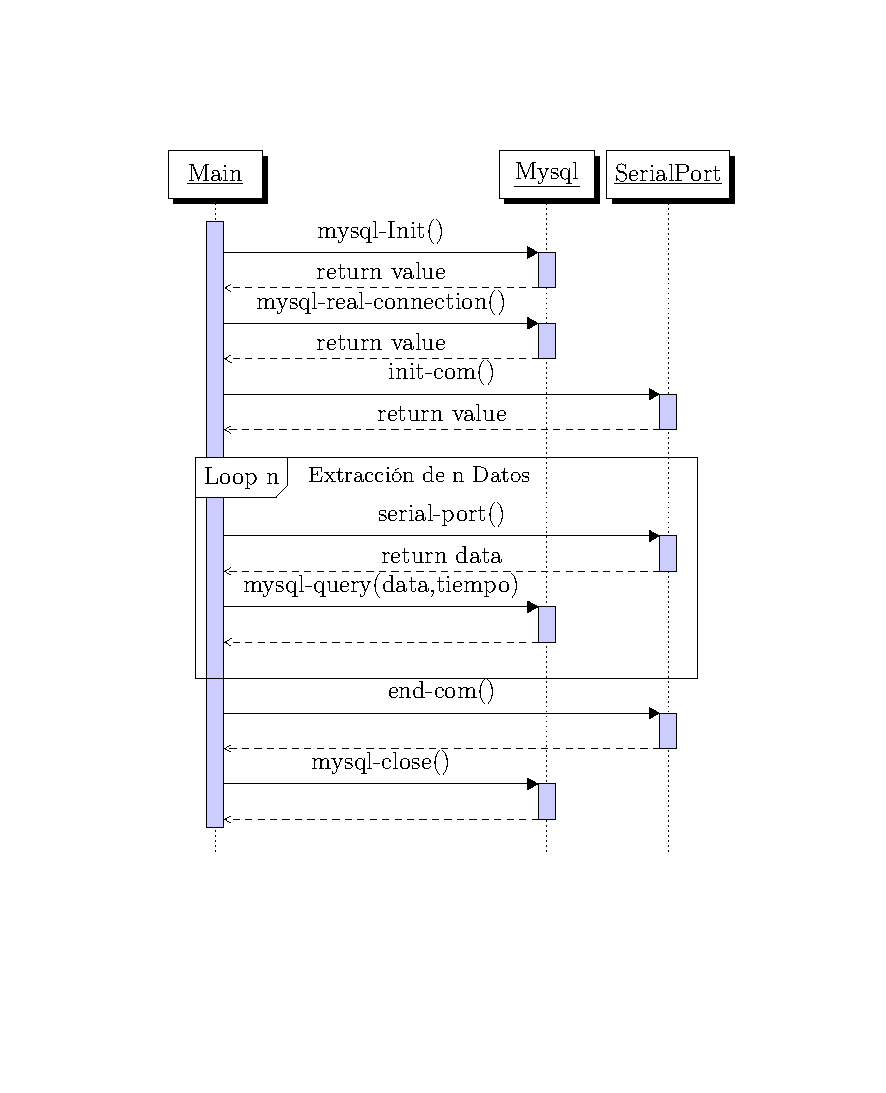
\includegraphics[width=1\textwidth]{./Cap5imagen/c.pdf}
	\caption[Diagrama de Secuencia Firmware OBDII.]{Diagrama de Secuencia Firmware OBDII \textbf{ Fuente:} Elaboración Propia.}
	\label{sobd} % Etiqueta para la referencia.
\end{figure}

%%%%%%%%%%%%%%%%%%%%%%%%


\subsection{Diseño del Firmware para el sistema J1939}

Para presentar la secuencia del procedimiento del protocolo J1939 nos apoyamos del diagrama de secuencia vista en la Figura~\ref{sj}.
Las partes más importantes son inicializar el módulo CAN, el módulo serial, el Timer2 y se habilitan las interrupciones necesarias. 
El {\bfseries timer2()} se utiliza como temporizador para medir los tiempos de comunicación con el bus. 
Se comienza con la función {\bfseries j1939init()}, dicha función provee de un nombre y una dirección al dispositivo para que pueda conectarse a la red, además envía un ''Address claim'' para reclamar una dirección. 
Si dicho reclamo es exitoso podemos empezar la comunicación con cualquier dispositivo, en caso contrario podemos cambiar automáticamente nuestra dirección e iniciar de nuevo el proceso hasta tener éxito. 
{\bfseries serial-init()} inicializa el puerto serial necesario para recibir y enviar información al servidor y con {\bfseries serial-isr() } recibimos los datos del servidor para indicar al microprocesador la lectura de los mensajes que deseamos del bus J1939. 

Una vez conectados se leen los mensajes presentes en el bus con la función {\bfseries J1939GetMessage()} y recuperamos el PGN (\textit{Parameter Group Number}, por sus siglas en inglés) , 
Dichos parámetros PGN pueden ser decodificados utilizando como referencia el documento SAE j1939-71 que nos proporciona las operaciones matemáticas para obtener la medición del sensor deseado.  
Todo ello se realiza con la función {\bfseries lecturaParametro()}.
Una vez leído y codificado pasamos los datos al servidor, con la cadena JSON  mediante la función {\bfseries print(JSON)}, dicho formato se representa como: 
\{
''PG'': ''F004'',
''DA'':  ''04'',
''SA'':  ''FF'',
''Data'' : [0,1,2,3,4,5,6,7],
''Value'': ''100''
\}

Donde PG significa Parámetro de Grupo, DA es Dirección de destino, SA dirección de origen, Data son los 8 bytes del bus can recibidos y ''Value'' es el dato calculado real para visualizar en el lado del cliente.





%%%%%%%%%%%%%%%%%%%%%%%%%%%%% DIAGRAMA DE SECUENCIA FIRMWARE j1939

\begin{figure}[t]
	\centering
	\begin{center}
		\begin {sequencediagram}
\newthread {main}{Main}


\newinst [1]{serial}{PuertoSerial}
\newinst [0]{name}{Init}
\newinst [1]{can}{BufferCAN}

\newinst [0]{pgn}{PGN}
\newinst [0]{int}{interrupción}
 

%%%%%enlaces%%%%%

\begin{call}{main}{J1939init()}{name}{true}
	\begin{call} 
		{name}{address claim}{can}{true-false}
	\end{call}
\end{call}

\begin{call}{main}{timer2()}{name}{true}
\end{call}

\begin{call}{main}{serial-init()}{name}{true}
\end{call}

\begin{call}{main}{serial-isr()}{int}{return PID}
\end{call}


\begin{sdblock}[blue!10]{Loop}{}

	\begin{call}[2]{main}{j1939GetMessage()}{can}{return data}
	\end{call}
	
	\begin{call}[2]{main}{lecturaParametro}{pgn}{true}\end{call}
    
    \begin{call}[2]{main}{print(JSON)}{serial}{void}
	\end{call}
    
    
	\end{sdblock}
\end {sequencediagram}
	\end{center}
	%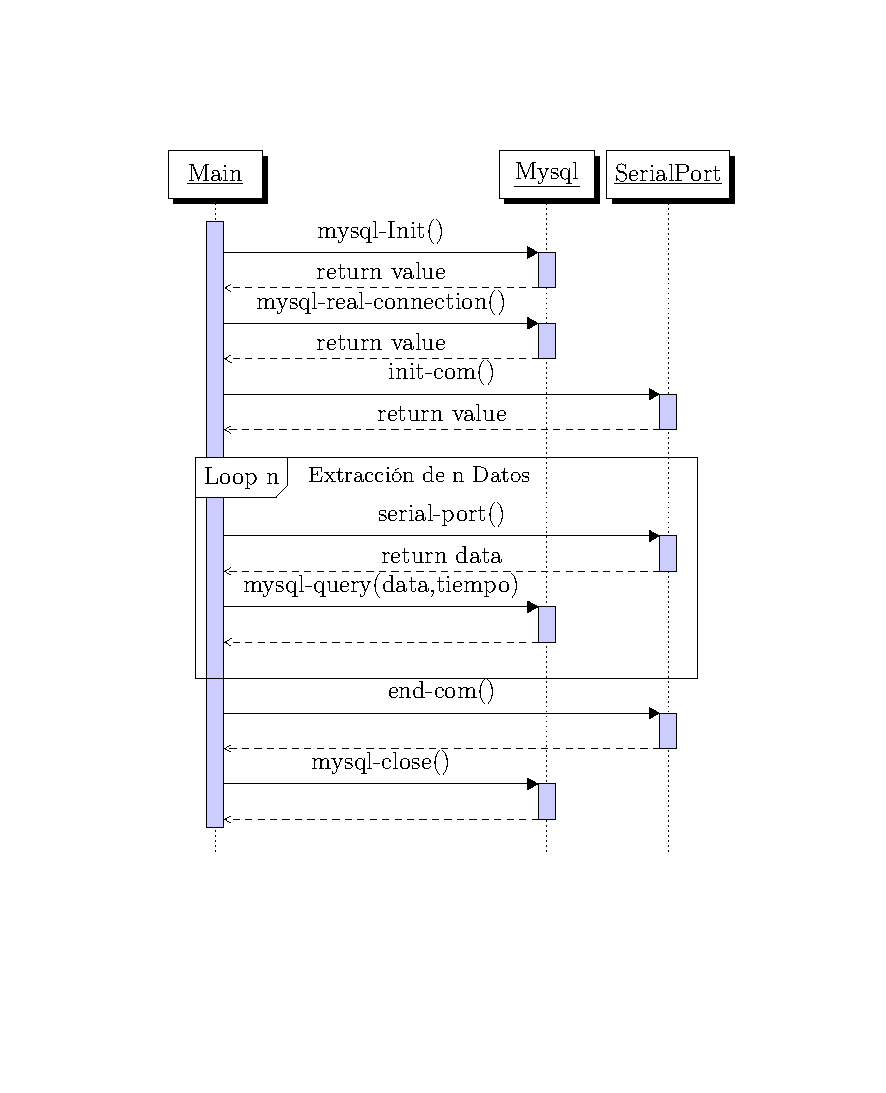
\includegraphics[width=1\textwidth]{./Cap5imagen/c.pdf}
	\caption[Diagrama de Secuencia Firmware OBDII.]{Diagrama de Secuencia Firmware OBDII \textbf{ Fuente:} Elaboración Propia.}
	\label{sj} % Etiqueta para la referencia.
\end{figure}

%%%%%%%%%%%%%%%%%%%%%%%%

\subsection{Diseño del Servidor BUS CAN}
En la \textbf{Figura~\ref{snode}} se detalla el diagrama de secuencia del sistema servidor BUS CAN, para el funcionamiento del programa requeriremos los módulos de http(), express(), y socket(). Una vez inicializados escuchamos el puerto socket para encontrar conexiones al sistema y al mismo tiempo escuchamos el puerto serial con {\bfseries parser.on()} por el cual se recibe datos del vehículo mediante el dispositivo CAN. 
Una vez detectada una conexión web del cliente,  el servidor  procede a enviar los datos del puerto serial al cliente mediante la conexión  {\bfseries socket.emit()}. Estos datos son enviados en formato JSON para un mejor procesamiento de los mismos,  así el cliente recibe constantemente los datos actualizados del vehículo automotor. 

%%%%%%%%%%%%%%%%%%%%%%%%%%%%% DIAGRAMA DE SECUENCIA SERVIDOR

\begin{figure}[t]
	\centering
	\begin{center}
		%%%%%%%%%%%%%%%%%%%%%%%%%%%%%%%%%%%%%%%%%%%%
\begin {sequencediagram}

\newthread [blue!20] {main}{main}
\newinst [1]{require}{Require}
\newinst [1]{serial}{PortSerial}
\newinst [1]{socket}{Socket}
\newinst [2]{cliente}{Cliente}


\begin{call} {main}{call}{require}{http()}
\end{call}

\begin{call}{main}{call}{require}{express()}
 \end{call}

 \begin{call}[1]{main}{call}{require}{socket()}
 \end{call}

\begin{call} {main}{parser.on()}{serial}{True}
	\begin{call}{serial}{socket.emit()}{socket}{true}
			\begin{call}{socket}{data(JSON)}{cliente}{true}
			\end{call}
	\end{call}
	
\end{call}
\end {sequencediagram}
	\end{center}
	%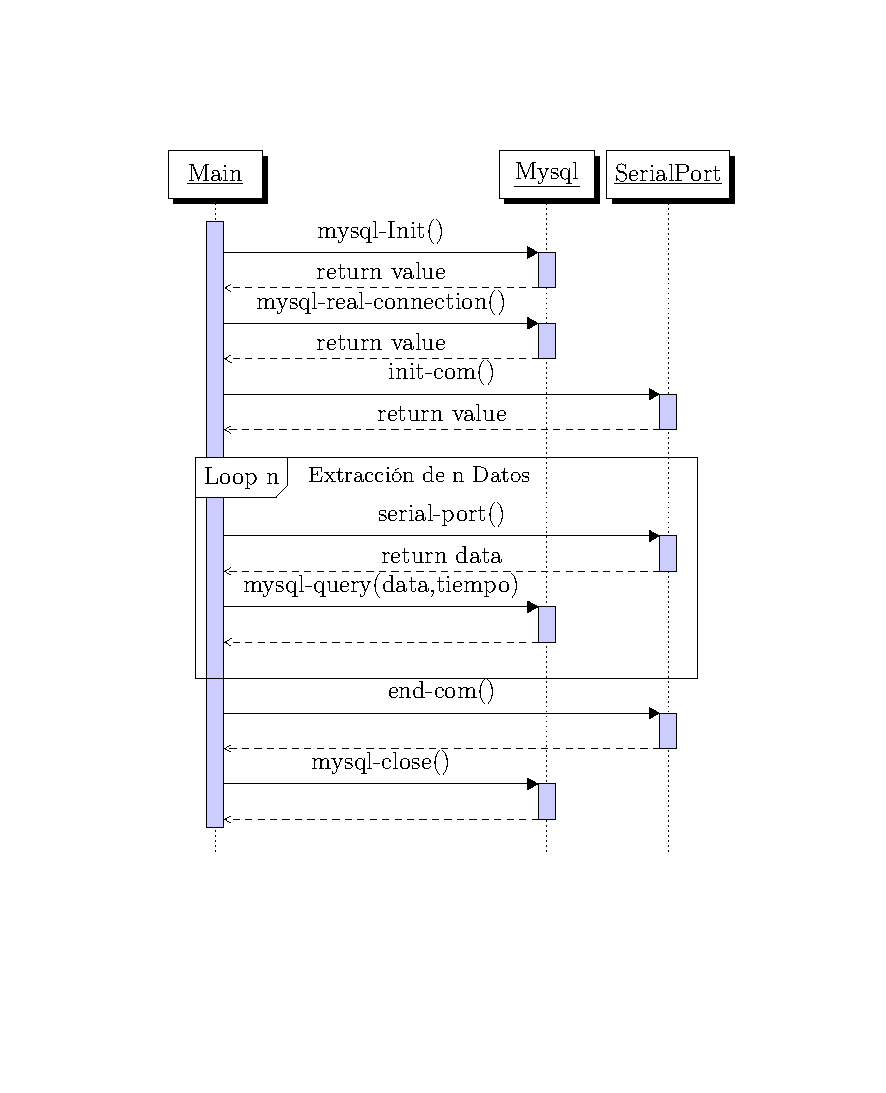
\includegraphics[width=1\textwidth]{./Cap5imagen/c.pdf}
	\caption[Diagrama de Secuencia Servidor CAN.]{Diagrama de Secuencia Servidor CAN \textbf{Fuente:} Elaboración Propia.}
	\label{snode} % Etiqueta para la referencia.
\end{figure}

%%%%%%%%%%%%%%%%%%%%%%%%




\subsection{Diseño de Software para el cliente de Interfaz de Datos BUS CAN}


Para la aplicación en el navegador se utiliza un script de  javascript del lado del cliente, este script visualiza los datos provenientes de la conección socket del servidor en una gráfica entendible para los usuarios. 
La función {\bfseries on()} de la librería socket.io se encarga de escuchar los datos provenientes del servidor y una vez recibidos pasamos dichos datos a las librerías de gráficos utilizadas y se corre un algoritmo de animación. 
Dichas librerías junto con el algoritmo se encargan de gestionar los datos para producir efectos de movimiento y experiencia de animación para el usuario. 
Estas funciones se ejecutan por cada dato recibido desde el servidor y cada 1 segundo, la función {\bfseries update(data)} se encarga de esta rutina de actualización. 
El siguiente diagrama en secuencia en la \textbf{Figura \ref{cweb}} detalla la situación: 
%%%%%%%%%%%%%%%%%%%%%%%%%%%%% DIAGRAMA DE SECUENCIA CLIENTE

\begin{figure}[H]
	\centering
	\begin{center}
		%%%%%%%%%%%%%%%%%%%%%%%%%%%%%%%%%%%%%%%%%
\begin {sequencediagram}

\newthread [blue!20] {web}{Main}
\newinst [1]{socket}{Socket}
\newinst [1]{chart}{Chart}

\newinst [3]{servidor}{Servidor}

%\begin{call}[1]{call} {}{}{}{}\end{call}
\begin{call}[1]{web}{on()}{socket}{data}
	\begin{call}[1]{socket}{socket.on()}{servidor}{data(JSON)}\end{call}
\end{call}

\begin{sdblock}[blue!10]{SetInterval}{Cada 1000ms}
	\begin{call}[1]{web}{update(data)}{chart}{true}\end{call}
\end{sdblock}

\end {sequencediagram}
	\end{center}
	%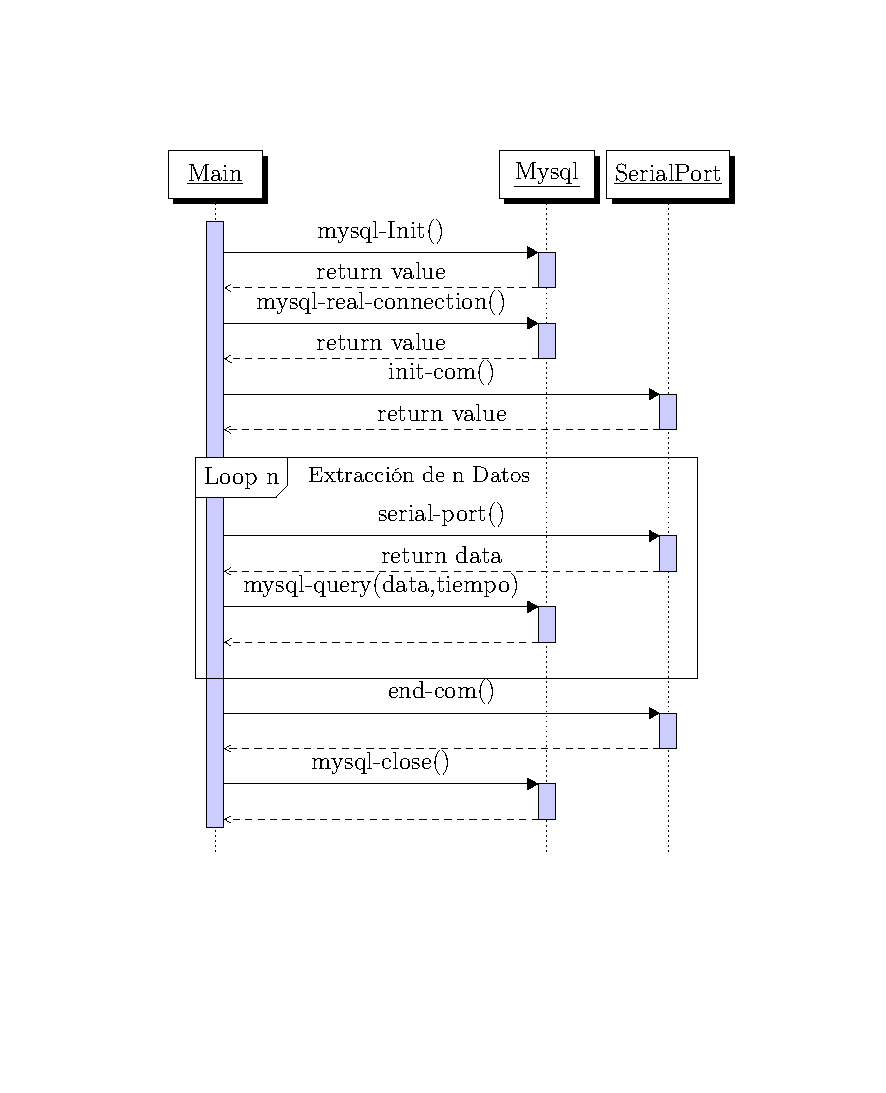
\includegraphics[width=1\textwidth]{./Cap5imagen/c.pdf}
	\caption[Diagrama de Secuencia Cliente Web.]{Diagrama de Secuencia Cliente Web \textbf{ Fuente:} Elaboración Propia.}
	\label{cweb} % Etiqueta para la referencia.
\end{figure}

%%%%%%%%%%%%%%%%%%%%%%%%
%%%%%%%%%%%%%%%%%%%%%%%%%%%%diagrama cliente
	

%%%%%%%%%%%%%%%%%%%%%%%%%%%%%inserta el diagrama

 
%%%%%%%%%%%%%%%%%%%%%%%%%%%

%%%%%%%%%%%%%%%%%%%%%%%%%%%%



%%% GITHUG
Los códigos del proyecto se encuentra en los siguientes repositorios de github, además de sus correspondientes archivos ``readme", que indican los pasos para su utilización: 
\begin{itemize}
    \item Desarrollo del Hardware prototipo para el manejo del protocolo BUS CAN:
   
   \url{https://github.com/JuanOrtizG/Prototipo-Hardware-CAN.git}
    \item Códigos del mircroprocesador PIC18F4580 para el sistema OBD II:
   
    \url{https://github.com/JuanOrtizG/canBusPic.git}
    \item Códigos del microprocesador PIC18F4580 para el sistema J1939: 
   
    \url{https://github.com/JuanOrtizG/canBusPic_J1939.git}
    \item Códigos del servidor para el sistema de visualización de datos: 
   
    \url{https://github.com/JuanOrtizG/nodeCan.git}
\end{itemize}



















